\chapter{State of the Art}
\label{cha:state_of_the_art}

% TODO: Add chapter introduction

\section{Analysis of and Contributions to the C\&M Literature}

% In this chapter the (about 3 (BT) / 6 (MT)) publications with a high relevance for the thesis are described.
% Publications which do have no or only a weak relationship with the thesis should not be part of this chapter.
% The C\&M LITERATURE is the source and destination of all literature work at C\&M.

% TODO: Do

\begin{figure}[bth]
    \centering
    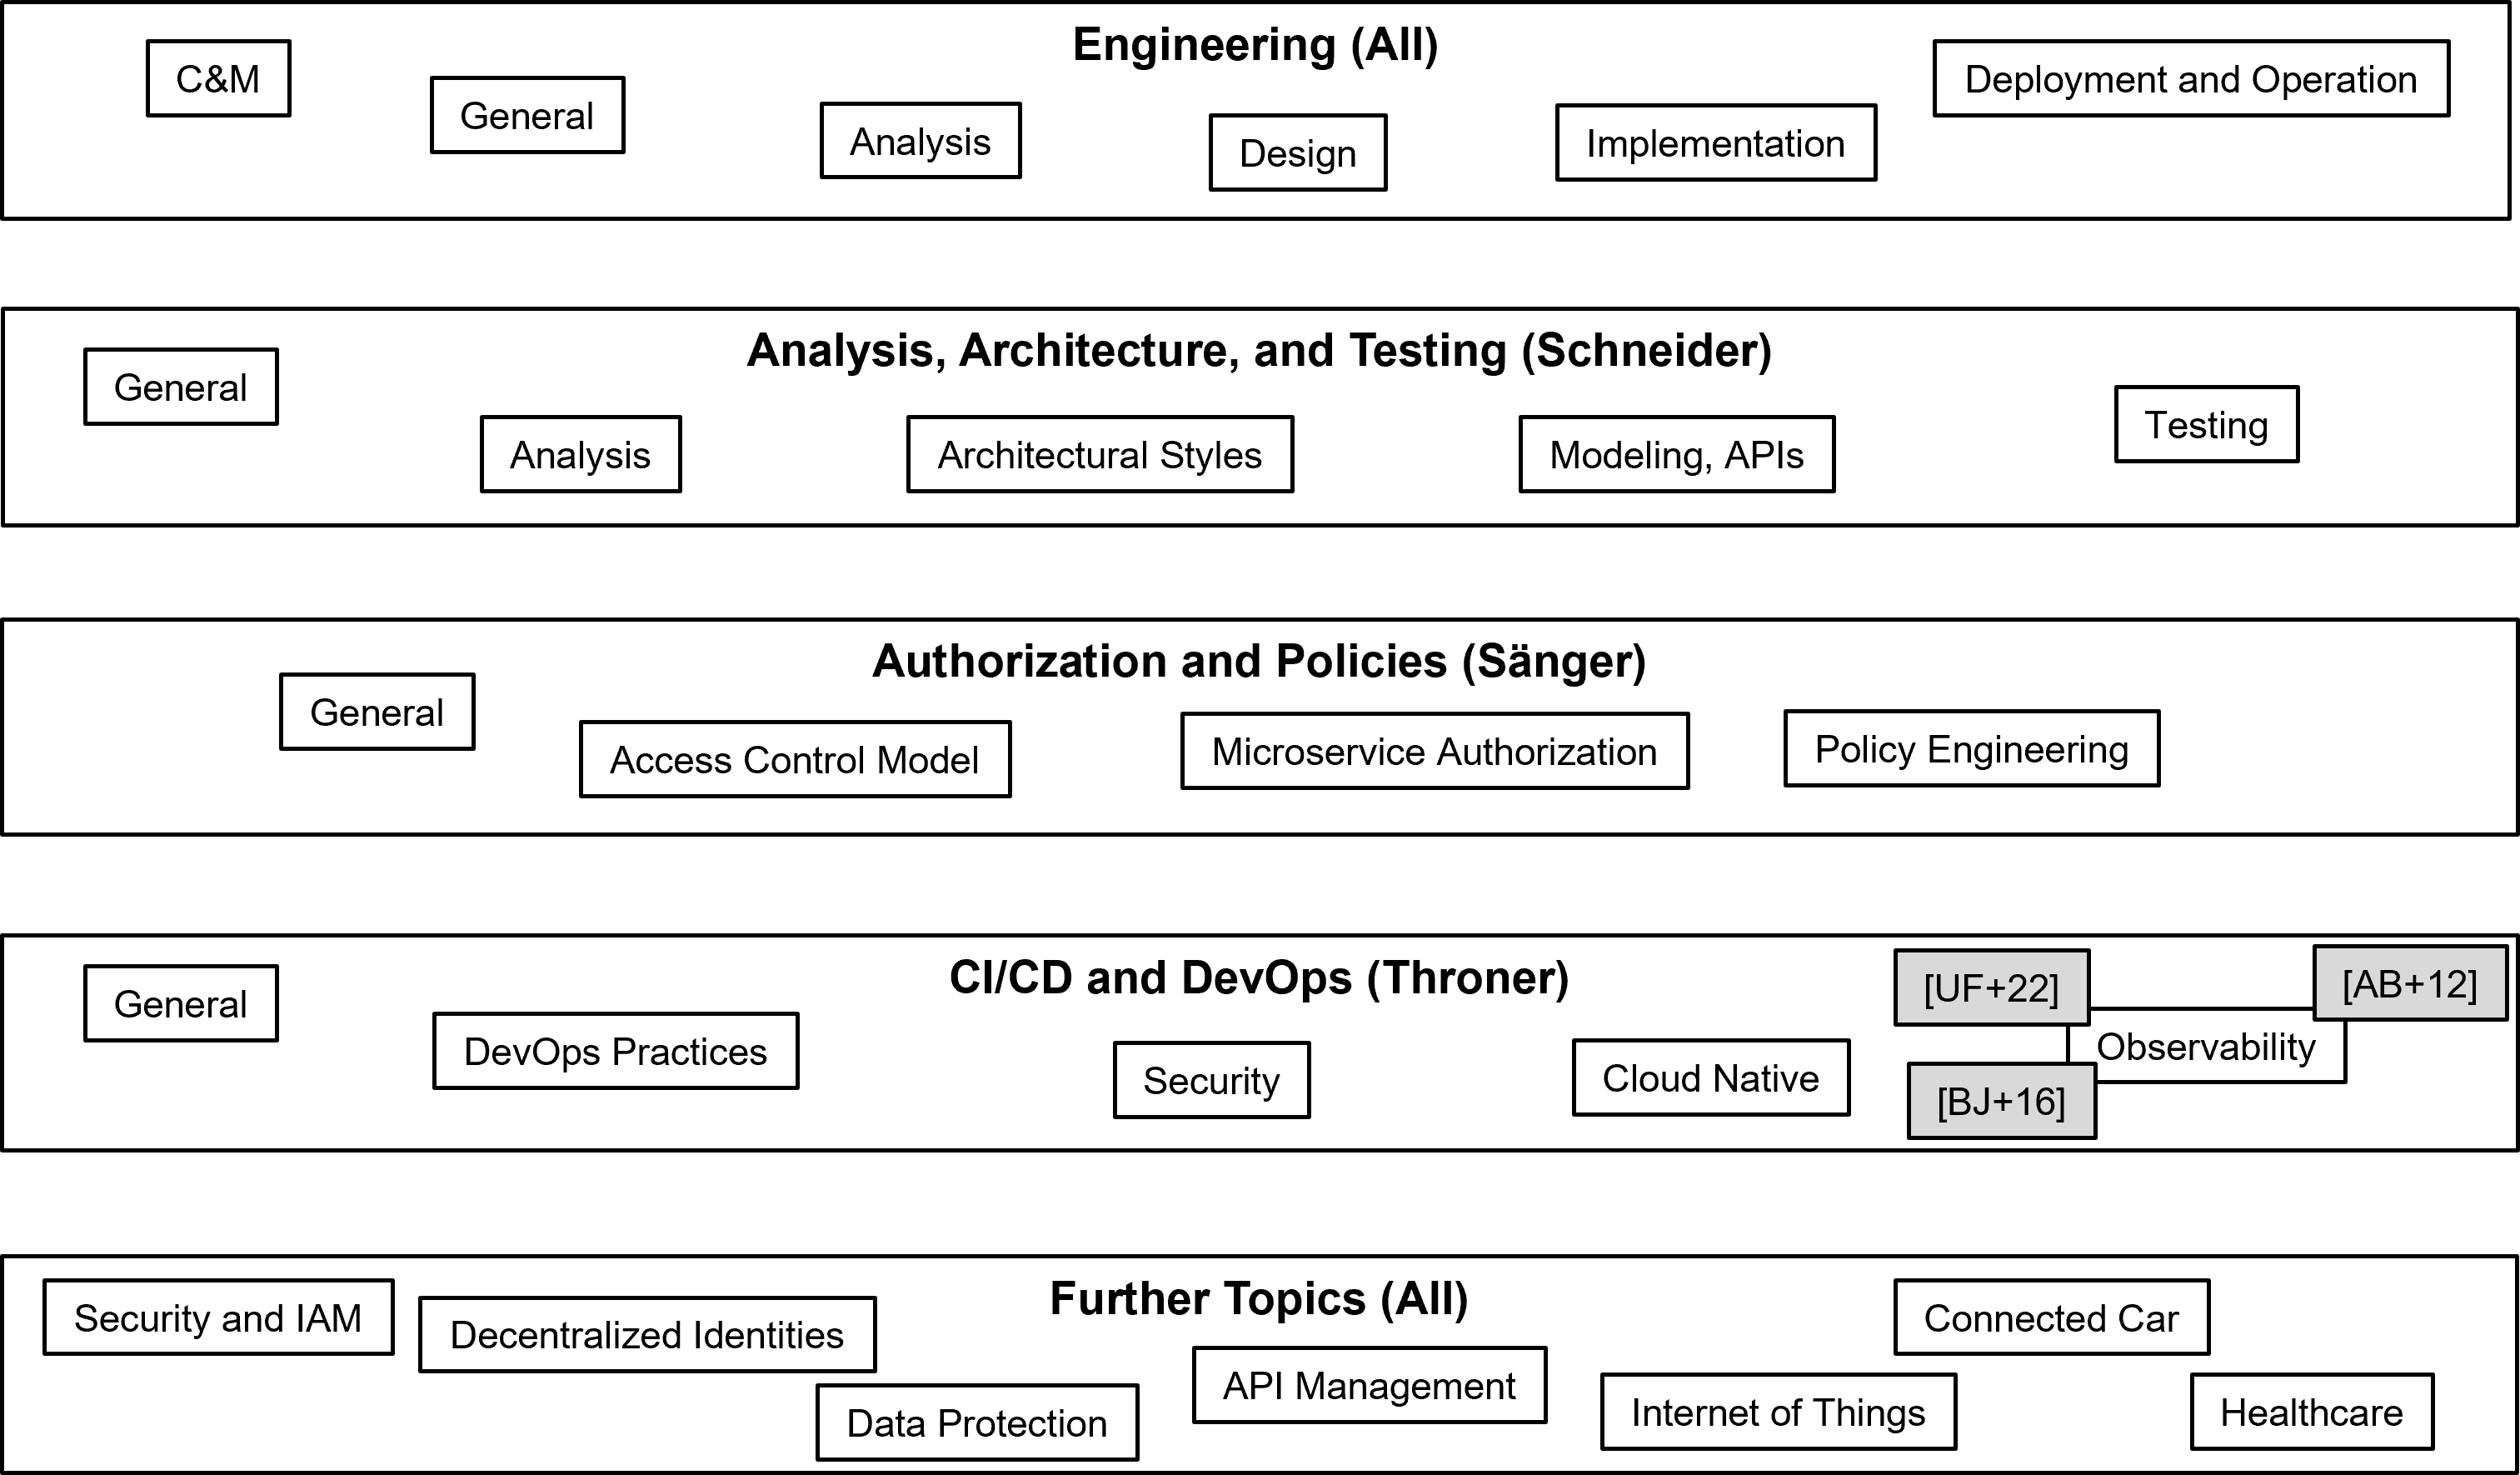
\includegraphics[width=\linewidth]{figures/literature.png}
    \caption{Categories and Subcategories}
    \label{fig:categories_subcategories}
\end{figure}

\subsection*{A Survey on Observability of Distributed Edge \& Container-Based Microservices \cite{UF+22}}
% This is the textbook on Domain-Driven Design (DDD) written by the DDD founder, Eric Evans.
% Core parts covered by this textbook can be found in those parts of the WASA course units \cite{CM-W-WAS}
% dealing with the design of web applications.
% It should be noticed that Evans developed the DDD concept in 2003 independently from the microservices
% which only came up about ten years later (for this reason the textbook is not grouped into this category).

% TODO: Do

Status: CREATE (the publication should become a part of the C\&M LITERATURE  (09.09.2023))

\subsection*{Site Reliability Engineering \cite{BJ+16}}

% TODO: Do

Status: CREATE (the publication should become a part of the C\&M LITERATURE  (09.09.2023))

\subsection*{Cloud monitoring: Definitions, issues and future directions \cite{AB+12}}

% TODO: Do

Status: CREATE (the publication should become a part of the C\&M LITERATURE  (09.09.2023))

% In the following sections, the 1 to 2 (BT) / 2 to 4 (MT) publications
% which have the highest influence on the solution worked out in this thesis
% are described in more detail (about 2 pages).
% The focus of the description should be set on the relationship of these publications
% to the thesis.

\section{Usman et al.: A Survey on Observability of Distributed Edge \& Container-Based Microservices}
\label{sec:uf+22}

% TODO: Do